%-----------------------------------------------------------------------
% Notes on Optimization with CgMx
%-----------------------------------------------------------------------
\documentclass[11pt]{article}
% \usepackage[bookmarks=true]{hyperref}  % this changes the page location !
\usepackage[bookmarks=true,colorlinks=true,linkcolor=blue]{hyperref}

\hbadness=10000 
\sloppy \hfuzz=30pt

\usepackage{calc}
\usepackage[lmargin=.75in,rmargin=.75in,tmargin=.75in,bmargin=.75in]{geometry}

\usepackage{amsmath}
\usepackage{amssymb}

\usepackage{verbatim}
\usepackage{moreverb}

\usepackage{graphics}    
\usepackage{calc}
\usepackage{ifthen}
\usepackage{float}
% the next one cause the table of contents to disappear!
% * \usepackage{fancybox}

\usepackage{tikz}
\input tex/trimFig.tex

\usepackage{listings}
\lstset{
basicstyle=\scriptsize\ttfamily,
columns=flexible,
breaklines=true,
commentstyle=\color{red},
keywordstyle=\color{black}\bfseries,
keepspaces=true
}

\input tex/defs

\newcommand{\bahDir}{/Users/henshaw/DropBox/EM_Homogenization/notes}

% *** See http://www.eng.cam.ac.uk/help/tpl/textprocessing/squeeze.html
% By default, LaTeX doesn't like to fill more than 0.7 of a text page with tables and graphics, nor does it like too many figures per page. This behaviour can be changed by placing lines like the following before \begin{document}

\renewcommand\floatpagefraction{.99}
\renewcommand\topfraction{.99}
\renewcommand\bottomfraction{.99}
\renewcommand\textfraction{.01}   
\setcounter{totalnumber}{50}
\setcounter{topnumber}{50}
\setcounter{bottomnumber}{50}

\begin{document}


\vspace{5\baselineskip}
\begin{flushleft}
{\LARGE
Notes on Optimization using Cgmx \\
}
\vspace{2\baselineskip}
William D. Henshaw, \\
% Derek Olson, \\
% Michael Jenkinson, \\
\large Extreme team ...\\
% 
\vspace{1\baselineskip}
% 
Department of Mathematical Sciences, \\
Rensselaer Polytechnic Institute (RPI), \\
Troy, NY, USA, 12180. \\
\vspace{\baselineskip}
\today\\

\vspace{4\baselineskip}

\noindent{\bf\large Abstract:}


This document describes the using the Overture CgMx time-domain Maxwell solver for optimization problems.
The initial version uses some simple optimization routines from Matlab. 
% 
% various dielectric bodies using Overture's {\tt Cgmx} time-domain solver for
% Maxwell's equations~\cite{CgmxUserGuide}. 

\end{flushleft}

% \clearpage
\tableofcontents
% \listoffigures

\clearpage
\section{Introduction}

We consider using the time-domain solver for Maxwell's equations, CgMx~\cite{CgmxUserGuide} to solve some optimization problems.


The optimizer is built with a few Matlab functions: 
\begin{itemize}
  \item {\tt optimizer.m} : simple optimizer using Matlab functions.
  \item {\tt runMaxwell.m} : run CgMx for a given case, and given parameters, and return appropriate results.
\end{itemize}



% ================================================================================================================
\clearpage
\section{Minimizing the reflection coefficient of a slab} \label{sec:reflectionAndTransmission}
Consider a dielectric block with $(\eps_1,\mu_1)$ occupying the region $x\in[-W/2,W/2]$ embedded in a material with $(\eps,\mu)$. 


{
% ---------------------------------------
%
\begin{figure}[hbt]
\newcommand{\textFont}{\normalss}
\begin{center}
 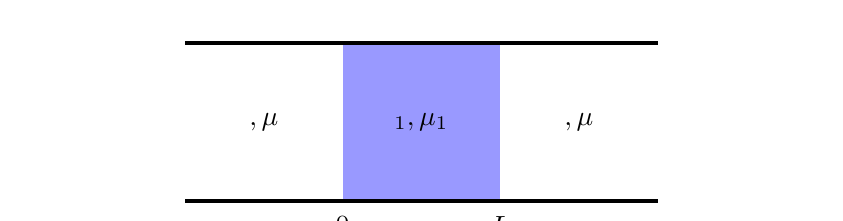
\begin{tikzpicture}[scale=1]
  %
  \useasboundingbox (0,.1) rectangle (10,2.2);  % set the bounding box (so we have less surrounding white space)
  %
  \begin{scope}[xshift=5cm,yshift=1cm]
   \fill[color=blue!40] (-1,-1) rectangle (1,1);
   \draw[-,line width=1.5pt] (-3, 1) -- (3, 1); %
   \draw[-,line width=1.5pt] (-3,-1) -- (3,-1); %
   %
   \draw ( -2,0) node[] {\textFont $\eps,\mu$}; 
   \draw ( 0,0) node[] {\textFont $\eps_1,\mu_1$}; 
   \draw (  2,0) node[] {\textFont $\eps,\mu$}; 
   %
   \draw (-1,-1) node[anchor=north,yshift=-2pt] {\textFont$0$}; 
   \draw ( 1,-1) node[anchor=north,yshift=-2pt] {\textFont$L$}; 
  \end{scope}
%-   %
% grid:
 % \draw[step=1cm,gray] (0,0) grid (10,4.);
  %
  \end{tikzpicture}
\end{center}
\caption{Dielectric block.}
\label{fig:dielectricBlock}
\end{figure}
}

{% ------ GRID AND TIME SEQUENCE CONTOURS  ------  
%
\newcommand{\figWidth}{12cm}% width
\newcommand{\trimfig}[2]{\trimwb{#1}{#2}{.0}{.0}{.35}{.4}}
\begin{figure}[htb]
\begin{center}
\begin{tikzpicture}[scale=1]
  \useasboundingbox (0,0.5) rectangle (12,9);  % set the bounding box (so we have less surrounding white space)

   \draw(0.0,6.0) node[anchor=south west,xshift=-15pt,yshift=-8pt] {\trimfig{\bahDir/fig/dieBlockG2}{\figWidth}};
   \draw(0.0,3.0) node[anchor=south west,xshift=-15pt,yshift=-8pt] {\trimfig{\bahDir/fig/dieBlockt0p0Ey}{\figWidth}};
   \draw(0.0,0.0) node[anchor=south west,xshift=-15pt,yshift=-8pt] {\trimfig{\bahDir/fig/dieBlockt3p0Ey}{\figWidth}};
% grid:
% \draw[step=1cm,gray] (0,0) grid (16,9);
\end{tikzpicture}
\end{center}
  \caption{Grid and sample solutions for the dielectric block, $k_x=1$, $\eps=8$.}
  \label{fig:dielectrciBlockGridAndContours}
\end{figure}
}



% ------------------------------------------------------------------------------------------
\subsection{Minimizing the reflection coefficient of a slab by varying $\eps_1$}

For this example we attempt to find the value of $\eps_1$ that  minimizes the reflection coefficient.
The analytic solution has one minimum at $\eps_1=4$ for this case (there are others, see Fig.\ref{fig:dielectricBlockCoeffVerusEps}). 

{% ------ REFLECTION AND TRANSMISSION VERSUS EPS2 ------  
%
\newcommand{\figWidth}{7.8cm}% width
\newcommand{\trimfig}[2]{\trimw{#1}{#2}{.0}{.0}{.0}{.0}}
\begin{figure}[htb]
\begin{center}
\begin{tikzpicture}[scale=1]
  \useasboundingbox (0,0.5) rectangle (8,7);  % set the bounding box (so we have less surrounding white space)

%   \draw(0.0,0.0) node[anchor=south west,xshift=-15pt,yshift=-8pt] {\trimfig{fig/dielectricBlockTransmissionCoeffVersusEpsL0p25}{\figWidth}};
   \draw(0.0,0.0) node[anchor=south west,xshift=-15pt,yshift=-8pt] {\trimfig{fig/dielectricBlockTransmissionCoeffVersusEpsL0p5}{\figWidth}};
% grid:
% \draw[step=1cm,gray] (0,0) grid (16,7);
\end{tikzpicture}
\end{center}
\caption{Dielectric block: reflection and transmission coefficients versus $\eps_1$ for $W=.5$ from
     the analytic solution.}
  \label{fig:dielectricBlockCoeffVerusEps}
\end{figure}
}


\noindent\textbf{Notes:}
\begin{enumerate}
  \item the incident plane wave has a wave number of $k_x=1$.
  \item the width of the slab is $W=.5$ (the grid actually occupies $x\in[-.25,.25]$). 
  \item the grid can be made with the Makefile ({\tt make dielectricBlock2d}). 
  \item a special {\em user defined probe} is used in this case that estimates the reflection and transmission coefficients. 
  \item  Typical output from a CgMx run is shown in Fig.~\ref{fig:dielectrciBlockRT} where the reflection and transmission
    coefficients are shown over time. Once the solution has reached a near time-periodic state the coefficients become
      constant in time. 
\end{enumerate}

% A typical numerical solution is shown in Fig.\ref{??}. 

{% ------ REFLECTION AND TRANSMISSION  ------  
%
\newcommand{\figWidth}{7.8cm}% width
\newcommand{\trimfig}[2]{\trimw{#1}{#2}{.0}{.0}{.0}{.0}}
\begin{figure}[htb]
\begin{center}
\begin{tikzpicture}[scale=1]
  \useasboundingbox (0,0.5) rectangle (8,7);  % set the bounding box (so we have less surrounding white space)

%   \draw(0.0,0.0) node[anchor=south west,xshift=-15pt,yshift=-8pt] {\trimfig{fig/dielectricBlockTransmissionCoeffVersusEpsL0p25}{\figWidth}};
   \draw(0.0,0.0) node[anchor=south west,xshift=-15pt,yshift=-8pt] {\trimfig{fig/blockReflectionTransmission}{\figWidth}};
% grid:
% \draw[step=1cm,gray] (0,0) grid (16,7);
\end{tikzpicture}
\end{center}
\caption{Dielectric block: reflection and transmission coefficients versus time as computed by CgMx.
Shown are the real and imaginary parts of $R$ and $T$, along with their magnitudes. 
   The magnitude of the
  reflection coefficient
  at the final time is optimized. 
}
  \label{fig:dielectrciBlockRT}
\end{figure}
}



\noindent Here is the output from {\tt optimizer.m} with messages from the Matlab function {\tt fminsearch}.  A value
of $\eps_1=3.975$ is obtained satisfying the tolerances. 

{\footnotesize
\begin{verbatim}
>>> optimizer: caseName=block, method=fminsearch, infoLevel=0, plotOption=1, tFinal=1.000e+01, probeType=transmission, 
call fminsearch...
runMaxwell: caseName=block, tFinal=1.000e+01 probeType=transmission, eps1=3, kx=1 
 
 Iteration   Func-count     min f(x)         Procedure
     0            1         0.394126         
runMaxwell: caseName=block, tFinal=1.000e+01 probeType=transmission, eps1=3.15, kx=1 
     1            2         0.364856         initial simplex
runMaxwell: caseName=block, tFinal=1.000e+01 probeType=transmission, eps1=3.3, kx=1 
runMaxwell: caseName=block, tFinal=1.000e+01 probeType=transmission, eps1=3.45, kx=1 
     2            4           0.2733         expand
runMaxwell: caseName=block, tFinal=1.000e+01 probeType=transmission, eps1=3.75, kx=1 
runMaxwell: caseName=block, tFinal=1.000e+01 probeType=transmission, eps1=4.05, kx=1 
     3            6        0.0297798         expand
runMaxwell: caseName=block, tFinal=1.000e+01 probeType=transmission, eps1=4.65, kx=1 
runMaxwell: caseName=block, tFinal=1.000e+01 probeType=transmission, eps1=3.75, kx=1 
     4            8        0.0297798         contract inside
runMaxwell: caseName=block, tFinal=1.000e+01 probeType=transmission, eps1=4.35, kx=1 
runMaxwell: caseName=block, tFinal=1.000e+01 probeType=transmission, eps1=3.9, kx=1 
     5           10        0.0297798         contract inside
runMaxwell: caseName=block, tFinal=1.000e+01 probeType=transmission, eps1=4.2, kx=1 
runMaxwell: caseName=block, tFinal=1.000e+01 probeType=transmission, eps1=3.975, kx=1 
     6           12         0.015101         contract inside
 
Optimization terminated:
 the current x satisfies the termination criteria using OPTIONS.TolX of 1.000000e-01 
 and F(X) satisfies the convergence criteria using OPTIONS.TolFun of 1.000000e-01 

...DONE fminsearch: x=3.975, fval=0.015101
\end{verbatim}
}

% ------------------------------------------------------------------------------------------
\subsection{Minimizing the reflection coefficient of a slab by varying the width}

For this example we attempt to find the value of the block width $W$ that  minimizes the reflection coefficient.
The analytic solution has one minimum at $W=.5$ for this case (there are others).

\medskip\noindent
Here is the output of a run. The optimizer {\tt fminsearch} finds the value of $W=.495$ satisfying the
tolerances. 

\begin{lstlisting}[frame=single,caption={blockWidth}]
>> optimizer -caseName=blockWidth -probeType=transmission -tf=10 -infoLevel=0 -method=fminsearch -blockWidth=.45
>>> optimizer: caseName=blockWidth, method=fminsearch, infoLevel=0, plotOption=1, gridFactor=4, tFinal=1.000e+01, probeType=transmission, 
             : kx=1, blockWidth=0.45, eps1=4
call fminsearch...
runMaxwell: caseName=blockWidth, RENGERATE THE GRID blockWidth=0.45
runMaxwell: caseName=blockWidth, tFinal=1.000e+01 probeType=transmission, eps1=4, kx=1 blockWidth=0.45 
 
 Iteration   Func-count     min f(x)         Procedure
     0            1         0.401063         
runMaxwell: caseName=blockWidth, RENGERATE THE GRID blockWidth=0.4725
runMaxwell: caseName=blockWidth, tFinal=1.000e+01 probeType=transmission, eps1=4, kx=1 blockWidth=0.4725 
     1            2          0.24439         initial simplex
runMaxwell: caseName=blockWidth, RENGERATE THE GRID blockWidth=0.495
runMaxwell: caseName=blockWidth, tFinal=1.000e+01 probeType=transmission, eps1=4, kx=1 blockWidth=0.495 
runMaxwell: caseName=blockWidth, RENGERATE THE GRID blockWidth=0.5175
runMaxwell: caseName=blockWidth, tFinal=1.000e+01 probeType=transmission, eps1=4, kx=1 blockWidth=0.5175 
     2            4        0.0466456         reflect
runMaxwell: caseName=blockWidth, RENGERATE THE GRID blockWidth=0.5175
runMaxwell: caseName=blockWidth, tFinal=1.000e+01 probeType=transmission, eps1=4, kx=1 blockWidth=0.5175 
runMaxwell: caseName=blockWidth, RENGERATE THE GRID blockWidth=0.50625
runMaxwell: caseName=blockWidth, tFinal=1.000e+01 probeType=transmission, eps1=4, kx=1 blockWidth=0.50625 
     3            6        0.0466456         contract outside
 
Optimization terminated:
 the current x satisfies the termination criteria using OPTIONS.TolX of 1.000000e-01 
 and F(X) satisfies the convergence criteria using OPTIONS.TolFun of 1.000000e-01 

...DONE fminsearch: x=0.495, fval=0.0466456
\end{lstlisting}



% ================================================================================================================
\clearpage
\section{Adjusting the shape of a lens} \label{sec:optimizeLens}

In this example the shape of a {\em lens} is adjusted to achieve some objective. 
The curves defining the left and right edges of the lens
are defined with NURBS curves. The shape can be controlled by adjusting the control points of the NURBS.


{% ------ Target solution   ------  
%
\newcommand{\figWidth}{5cm}% height
\newcommand{\trimfig}[2]{\trimh{#1}{#2}{.15}{.15}{.35}{.35}}
\begin{figure}[htb]
\begin{center}
\begin{tikzpicture}[scale=1]
  \useasboundingbox (0,0.75) rectangle (13,5);  % set the bounding box (so we have less surrounding white space)

  \draw(0.0,0.0) node[anchor=south west,xshift=-15pt,yshift=-8pt] {\trimfig{fig/lensG4TargetSolution}{\figWidth}};
% grid:
%  \draw[step=1cm,gray] (0,0) grid (13,5);
\end{tikzpicture}
\end{center}
  \caption{Target lens shape and solution ($E_y$).}
  \label{fig:lensTarget}
\end{figure}
}

{% ------ GRID AND TIME SEQUENCE CONTOURS  ------  
%
\newcommand{\figWidth}{4.9cm}% width
\newcommand{\figWidtha}{8cm}% 
\newcommand{\trimfig}[2]{\trimw{#1}{#2}{.3}{.3}{.37}{.37}}
\newcommand{\trimfiga}[2]{\trimh{#1}{#2}{.3}{.35}{.0}{.1}}
\begin{figure}[htb]
\begin{center}
\begin{tikzpicture}[scale=1]
  \useasboundingbox (0,0.5) rectangle (16,8);  % set the bounding box (so we have less surrounding white space)
% 
   \draw(0.0,0.0) node[anchor=south west,xshift=-15pt,yshift=-8pt] {\trimfiga{fig/lensCurveWithControlPoints}{\figWidtha}};
%    
  \begin{scope}[xshift=4cm]
   \draw( 0.0,4.0) node[anchor=south west,xshift=-15pt,yshift=-8pt] {\trimfig{fig/lensGridIteration1}{\figWidth}};
   \draw( 0.0,0.0) node[anchor=south west,xshift=-15pt,yshift=-8pt] {\trimfig{fig/lensGridIteration4}{\figWidth}};
   \draw( 6.0,4.0) node[anchor=south west,xshift=-15pt,yshift=-8pt] {\trimfig{fig/lensGridIteration7}{\figWidth}};
   \draw( 6.0,0.0) node[anchor=south west,xshift=-15pt,yshift=-8pt] {\trimfig{fig/lensGridIteration10}{\figWidth}};
  \end{scope} 
% grid:
% \draw[step=1cm,gray] (0,0) grid (16,8);
\end{tikzpicture}
\end{center}
\caption{Left: Nurbs curve for lens shape with control points.
  Right: sequence of grids for optimization of the shape of a lens (adjusting the right face of the lens).}
  \label{fig:lensGridOptimization}
\end{figure}
}

Figure~\ref{fig:lensGridOptimization} shows the results of a simple test.
The code was first run with a given lens shape and the transmission coefficent (averaged over a box to the right of the lens)
was saved as the {\em target transmission coefficient} (see Figure~\ref{fig:lensTarget}). 
The objective of the optimization was then to start from a different lens shape and adjust the
central control point on the right face of the lens to match the target transmission coefficient. 

Here are the results from the optimizer using {\tt fminsearch}
{\footnotesize
\begin{verbatim}

\end{verbatim}
}


  

%- 
%- 
%- {% ------ GRID AND TIME SEQUENCE CONTOURS  ------  
%- %
%- \newcommand{\figWidth}{12cm}% width
%- \newcommand{\trimfig}[2]{\trimwb{#1}{#2}{.05}{.05}{.3}{.325}}
%- \begin{figure}[htb]
%- \begin{center}
%- \begin{tikzpicture}[scale=1]
%-   \useasboundingbox (0,0.5) rectangle (12,5);  % set the bounding box (so we have less surrounding white space)
%- 
%- %   \draw(0.0,3.0) node[anchor=south west,xshift=-15pt,yshift=-8pt] {\trimfig{\bahDir/fig/dieBlockt0p0Ey}{\figWidth}};
%- %   \draw(0.0,0.0) node[anchor=south west,xshift=-15pt,yshift=-8pt] {\trimfig{\bahDir/fig/dieBlockt3p0Ey}{\figWidth}};
%- % grid:
%- % \draw[step=1cm,gray] (0,0) grid (16,9);
%- \end{tikzpicture}
%- \end{center}
%-   \caption{Curve for lens shape with control points.}
%-   \label{fig:lensCurveWithControlPoints}
%- \end{figure}
%- }


% ================================APPENDIX =========================================================================
\appendix
\section{Matlab codes}

% ----------------------------------------------------------------------------------------------
\subsection{optimizer.m}
\lstinputlisting[language=Matlab, numbers=left, stepnumber=1, firstline=1,caption={optimizer.m},frame=single]{optimizer.m}

% ----------------------------------------------------------------------------------------------
\subsection{runMaxwell.m}
\lstinputlisting[language=Matlab, numbers=left, stepnumber=1, firstline=1,caption={runMaxwell.m},frame=single]{runMaxwell.m}

\clearpage
\bibliography{henshaw,henshawPapers}
\bibliographystyle{siam}



\end{document}
% **************************************************************************************************************
% **************************************************************************************************************
% **************************************************************************************************************
% **************************************************************************************************************









